\chapter{Related Products and Research} % Main chapter title

\label{chapter3} % For referencing the chapter elsewhere, use \ref{Chapter1} 

Self-monitoring through technology is still in it's early stages, some view it as a temporary interest that will fade over time, others look at this technology as an invaluable tool to help understand ourselves better. There is no denying that research, communities, and products have surfaced that aim to understand and provide help with self-monitoring. In this section we will start out by looking at the communities around the technology, and look at some of the existing products. Finally we will present earlier research done that is relevant to our thesis.

\section{Communities}
Currently there are two names that stand out within self-monitoring: Quantified Self, and Personal Informatics. Quantified self is a community of end users who share data and exchange experiences with tools that help them collect information. Personal Informatics on the other hand is academic and developer driven, they desire to understand what makes a good tool, and how the user interacts with such technology.

\subsection{Quantified Self}
In 2011 a movement known as Quantified Self*\cite{quantifiedSelf} had their first conference \cite{bodyHackers}, here people shared data that they had collected about themselves width different types of devices. The goal is to gather as much information about yourself as possible, to learn about yourself through quantitative data. Members of Quantified Self* collect information about everything from sleep patterns and diets to mood and stress levels.

%Is this better?
To promote further development in tools that gather these types of information, the participants of Quantified Self has worked closely with companies and individuals that create personal informatics tools. Devices such as Nike's FuelBand \cite{fuelBand} and Fitbit \cite{fitBit} are results of this cooperation, and both products have been well received.

%Maybe make it clearer that it is an exchange of information between QS and developers?
%The exchange of information within the movement between users and tool makers %Tool makers, really?
% allows for new, exciting and relevant technology to be developed. The FuelBand\cite{fuelBand}, Fitbit\cite{fitBit} are some of results of this cooperation, and both products seem to be well received by the movement.
 
\subsection{Personal Informatics}
Personal informatics is the label used to classify tools that help people collect personal information for the purpose of self-monitoring and self reflection. These tools are used to help individuals gain self-knowledge about their behaviour, habits, and thoughts\cite{personalInformatics}.

The Computer-Human Interaction (CHI) conference has since 2010 \cite{chi2010} held workshops and accepted papers on Personal Informatics. The aim is to increase understanding of how the tools affect the user, explore new possibilities, and overall improvement of the user experience.
	
\section{Products}
%Maybe something should be added here?
\subsection{Nike+}
The Nike+ concept has existed since 2010 and is the brand name Nike uses for sports related activity tracking. A sensor in the shoe and a receiver connected to an iPod was the first Nike+ product. Since then the Nike+ line has expanded into Kinect Games, sport watches and shoe implants \cite{nikeProducts}. As the product line increased so did the community around it. Every Nike+ device now requires an online profile where user can store information, create goals, and look at their history. However the Nike+ FuelBand \cite{fuelBand} is the first product aimed at monitoring the user outside of their workout, and motivating them to reach the daily activity goals.

FuelBand was released in early 2012 and was the first commercial wrist worn activity monitor. The wristband contains a 3-axis accelerometer that tracks the users wrist movement. Recorded activity is converted to \emph{Nikefuel} \cite{nikefuel}, NikeFuel is a unit of measurement used by all Nike activity trackers, however there are no details on how activity is converted to NikeFuel, as the algorithm is proprietary. The wristband does calculate steps and calories burned, but the NikeFuel is the prime focus of their product line. NikeFuel does not take into account gender, height, weight, but looks purely at activity. Meaning that a mile will award the same amount of points to users of very different physiology. The daily progress is represented through a ring that fills up when the FuelBand detects activity, the ring is full once the daily activity goal is reached. If the NikeFuel goal is exceeded by a certain percentage the ring will gain visual improvements. 

NEED IMAGE FROM REVIEW HERE! DO WE NEED APPROVAL!?%IMAGE HERE IF THEY GET APPROVED BY SVANÆS

The information from the FuelBand can be uploaded to an iPhone or laptop which then send the information to the Nike+ servers and update the users profile. The online profile provides detailed information of the users activity, showing steps, calories burned, active time, distance travelled and average fuel. Charts can be displayed for weeks, months or years. This allows the user to track their progress and look at how often they achieve or go way above their goals.\cite{fuelbandTechSpce}. 
 
NEED IMAGE FROM REVIEW HERE! DO WE NEED APPROVAL!?%SHOW ACTIVITY BREAKDOWN
 
Virtual trophies are awarded for various achievements such as gathering an X amount of NikeFuel or beating the set goal by a 100\%. These trophies can then be shared with friends or displayed on the public profile to show off achievements. The FuelBand can display simple information such as how far the user is from his daily goal, steps taken, and calories burned. A review has reported that the NikeFuel concept can almost become an addiction and lead to doing some last minute workouts in order to reach the goal \cite{fuelbandDcRain}.

%I agree that this might be a little too specific, since we are not using this technology.  %Unsure if specific technical details should be mentioned, such as that it communicates through bluetooth etc. I figure the relevancy of these products is more on how they do things and what we can learn.

\subsection{Fitbit}
The Fitbit concept wishes to be much more involved in the subjects daily life. While the Nike+ only tracks activity, Fitbit lets the user log their sleep, food, heart rate, blood pressure and glucose. It does not specifically target exercises, but instead allows the user to track their everyday life. The product line currently consists of the Zip, One, and Aria. The Zip and One are hip worn activity trackers and will automatically update the users online profile when synced. The automatic activity trackers count only steps, but other activities and even manual labour are supported and can be entered by the user. Fitbit One is also able to track stairs climbed, hours slept and sleep quality allowing this to be automatically tracked. Aria is the Fitbit scale, if the device is linked to an online profile it will automatically update BMI, Weight, and body fat percentage at each weighing. Currently there are no official Fitbit devices that track blood pressure, heart rate or calorie intake, these all have to be entered manually if the user wishes to do so. There is also a journal where the user can create entries to describe their day and rate their mood.

Similar to the Nike+ the Fitbit allows the user to set daily goals, but as the Fitbit does not use the NikeFuel system, it enables the user to set 3 separate goals: steps taken, floors climbed, and calories burned. The Fitbit does provide an active score, but there is no emphasis on it. A daily activity breakdown is provided, this breaks the activity levels for the day into 4 categories: sedentary, lightly active, fairly active, and very active. All the goal histories can be viewed on the online profile and can be categorized into day, week, months and years. This is also applicable to other measurements such sleep, mood, blood pressure and glucose levels. 

NEED IMAGE FROM REVIEW HERE! DO WE NEED APPROVAL!?

As goals are reached Fitbit members are awarded badges. These badges are very similar to the Trophies that Nike+ awards their users. It can either be for having a very active day or lifetime achievements such as accumulating over 50,000 steps. The user can choose if he wishes these badges to be public or personal, and can be displayed on the profile if desired.

The Flex is the first wrist worn activity monitor from Fitbit, and is slated for release in June 2013. It will have the same functionality as the Fitbit One, with the exception of an altimeter, meaning it can not measure stairs climbed. This is considered to be the greatest upcoming competitor for the Nike+ FuelBand.

%We should write about the many smartphone apps that offer self-tracking.
\section{Related Research}

%THIS SECTION NEEDS REVIEW!
\subsection{Stage-Based Model of Personal Informatics Systems}
When talking about personal informatics it is useful to divide the personal informatics system into stages. Ian Li et al. created a stage-based model (see figure~\ref{fig:stageModelPI}) \cite{li2010} with five different stages: \emph{preparation}, \emph{collection}, \emph{integration}, \emph{reflection}, \emph{action}. The preparation stage is the stage before actual data is collected. This stage describes how and why people are motivated to collect data about themselves, which data is to be collected, and how.Most elderly would not by them self be motivated to start collecting data about them selves. Healthcare personnel can be an important motivator in this regard, by explaining the concept and benefits of self-reflection. 

\begin{figure}[h!]
	\centering
		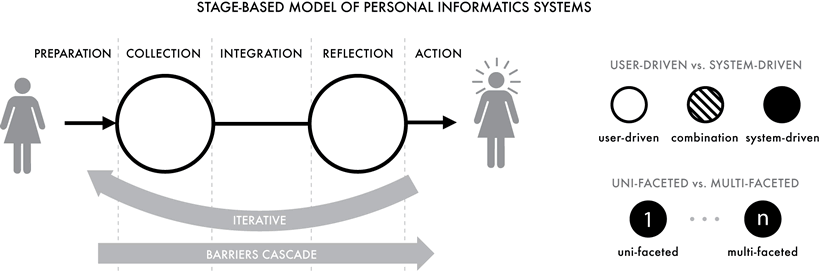
\includegraphics[width=0.5\textwidth]{stageModelPI.png}
		\caption{\footnotesize Taken from the Ian Li article \cite{li2010}}.
		\label{fig:stageModelPI}
\end{figure}

In the collection stage, data is collected. In this project all data collection was system driven, and the participants did not have to write down or be aware of their activity during this stage. Using a fully automated system will make it more attractive, since there is almost no effort connected to the collection of data. The sensor is small and barely noticeable.

The stage before reflection is the integration stage. This is the stage where the collected data is transformed into something that is useful. Creating visualizations is a powerful way to present large amount of data in a way that can be understood by humans in a short amount of time. 

In the reflection stage the users looks at the different charts to get an overview of the behavioural patters throughout the week. Since the data presented is collected over a longer period it is important that some time is used to analyse the data and identify patterns that may be instrumental in the last stage, action. Healthcare personnel can supervise the self-reflection and give explanations and instructions on how to interpret the different visualizations for best effect.

The last stage is the action stage. In this stage the user should change their behaviour to improve themselves. This stage is probably the most important, but also the hardest. For the users to improve they have to want to improve and they need to know how to improve. The reflection stage can help to identify periods of the day with long sedentary behaviour and with the help of the healthcare personnel a plan with concrete goals should be created. 

Ian Li et al. also identified a set of barriers for each of the five steps in the model. Barriers are problems that the participants of the study had when performing each step of the model. We will now list some of barriers that are applicable to our project, and how we aim to solve them. 

In the collection stage some of the most important barriers are having the right tools, remembering to collect data and lack of time. All of these barriers should be easily countered by the use of the activePAL sensor. Data is automatically recorded and the users does not have to do anything except wear the sensor and make sure not to break it while it is being uses. Using a fully system-driven approach in the collection stage give us more consistent and reliable data.

The integration stage is also mostly system-driven in our solution. The most important barriers for this step are related to transcribing and organizing data. Our program handles all the parsing and presents the data as different visualizations, so the transcribing will not be hard. Currently the application only handles a singe entry of data, and lets you see different visualizations of this data. Future work may be adding the possibility of comparing not only days, but weeks and months.

Notable barriers in the reflection stage are lack of time, visualizations, interpretation and self-criticism. Lack of time should not be to much of an issue for us, because the elderly population will most likely have more than enough time to participate in tests recommended to them by healthcare personnel. The visualization and interpretation barriers are central for our project. The goal of this project is to measure the effectiveness of different types of visualizations and discuss what types visualizations gives the most useful information as well as how easy they are to interpret. Self-criticism can also present a problem, some users may have a hard time looking at and reflecting over personal data. With the help and encouragement of healthcare personnel it is possible to minimize this problem. 

For the action stage it is critical that the users get motivated to change for the better, through reflecting on the data collected. It may also be helpful for the user to be provided with suggestions on how to improve their behavioural patterns. Tools could also be created to help remind the users to be more active, for example by adding reminders into calendars.

%This section is not written yet.
%Using this model Li %should I mention the others? Use et al.?
%came up with four recommendations for personal informatics systems. 
%\begin{quote}
%	Personal informatics systems should
%	1) be designed in a holistic manner across the stages.
%	2) allow iteration between stages.
%	3) apply an appropriate balance of automated technology and user control within each state to facilitate the user experience.
%	4) explore support for associating multiple facets of people's lives to enrich the value of the system.
%\end{quote}
